\documentclass[aspectratio=169,11pt]{beamer}
\usetheme{default}\usecolortheme{seahorse}
\setbeamertemplate{navigation symbols}{}
\setbeamertemplate{footline}[frame number]
\setbeamerfont{frametitle}{size=\large,series=\bfseries}
\setbeamercolor{frametitle}{fg=structure}
\setbeamertemplate{itemize items}[circle]
\setbeamertemplate{blocks}[rounded][shadow=false]
\usepackage[T1]{fontenc}\usepackage{lmodern}\usepackage{booktabs}
\usepackage{tikz}\usepackage{xcolor}
\usetikzlibrary{arrows.meta,positioning}
\definecolor{codebg}{HTML}{F4F4F4}\definecolor{keyc}{HTML}{1F77B4}
\definecolor{warnc}{HTML}{B03030}\definecolor{okc}{HTML}{2CA02C}
\definecolor{dimc}{HTML}{707070}
\newcommand{\file}[1]{\texttt{\small #1}}
\newcommand{\cue}[1]{\textbf{\color{keyc}#1}}
\usepackage{listings}
\lstset{basicstyle=\ttfamily\scriptsize,backgroundcolor=\color{codebg},
  frame=none,breaklines=true,columns=flexible,xleftmargin=6pt,
  framexleftmargin=6pt,aboveskip=4pt,belowskip=4pt}
\title{mjc\_sitl\_px4}
\begin{document}

{\setbeamertemplate{footline}{}
\begin{frame}
  \vspace{1.1cm}
  \begin{center}
    {\Huge\bfseries \texttt{mjc\_sitl\_px4}}\\[0.5cm]
    {\Large Three controllers, flown as ROS\,2 nodes}\\[1.0cm]
    {\large\color{dimc} PD, MPC and a trained PPO policy ---}\\[0.15cm]
    {\large\color{dimc} what runs, what does not, and how to run it.}
  \end{center}
\end{frame}}

% ---------------------------------------------------------------
\begin{frame}[fragile]{The problem}
  You write a drone controller in MuJoCo. It works. Now it has to run as a
  ROS\,2 node, because that is what runs on hardware.

  \vspace{0.4cm}
  The normal path is to open the MuJoCo script on one monitor, an empty ROS
  node on the other, and retype it.

  \vspace{0.4cm}
  \cue{That rewrite is where the bugs come from} --- not because people are
  careless, but because nothing checks the result. Two pieces of code that are
  meant to do the same thing, and no way to tell whether they do.

  \vspace{0.5cm}
  \begin{block}{What this does}
    Runs your controller in simulation, runs the \emph{same} controller through
    ROS\,2, and compares the two flights numerically.
  \end{block}
\end{frame}

% ---------------------------------------------------------------
\begin{frame}[fragile]{The demo}
\begin{lstlisting}
$ cd ~/mjc_sitl_px4
$ ./demo.sh show
\end{lstlisting}

  \vspace{0.3cm}
  Three recorded flights, figure-8, 24\,s, each through the real ROS\,2 stack:

  \vspace{0.25cm}
  \begin{center}
  \small
  \begin{tabular}{@{}lrrl@{}}
    \toprule
    & tracking RMSE & solve p95 & \\
    \midrule
    \textbf{PD}  & 0.119 m & 0.09 ms & position $\to$ tilt $\to$ torque\\
    \textbf{MPC} & \textbf{0.078 m} & 8.3 ms & convex QP, hover linearisation\\
    \textbf{PPO} & 0.133 m & 0.43 ms & residual policy over PD\\
    \bottomrule
  \end{tabular}
  \end{center}

  \vspace{0.3cm}
  {\small MPC tracks best and costs $\sim$90$\times$ more compute. PPO is worst
  here, which is expected --- with no wind, PD is already near-optimal on this
  task and a residual policy mostly adds exploration noise.}
\end{frame}

% ---------------------------------------------------------------
\begin{frame}[fragile]{Why they agree: one model, two harnesses}
  The ROS\,2 node does not have its own copy of the scene. It calls
  \file{sim\_mjc}'s own \file{build\_scene()} --- same function, same compiled
  MuJoCo model.

  \vspace{0.3cm}
  \begin{center}
  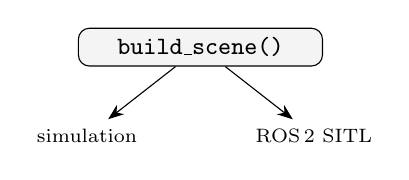
\begin{tikzpicture}[scale=0.9, every node/.style={font=\scriptsize}]
    \node[draw, rounded corners, fill=codebg, minimum width=3.1cm] (c) at (0,0.65)
      {\file{build\_scene()}};
    \node (d) at (-1.6,-0.6) {simulation};
    \node (e) at (1.6,-0.6) {ROS\,2 SITL};
    \draw[-{Stealth[length=2mm]}] (c) -- (d);
    \draw[-{Stealth[length=2mm]}] (c) -- (e);
  \end{tikzpicture}
  \end{center}

  \vspace{0.2cm}
  So the two differ only in transport, which step the command lands on, and
  executor jitter --- \cue{all properties of the deployment, none of physics.}

  \vspace{0.3cm}
\begin{lstlisting}
$ ./demo.sh parity
parity: OK (12/12 checks)
\end{lstlisting}

  \vspace{0.1cm}
  {\footnotesize Masses, inertias, gearing, thrust limits, timestep, allocation
  matrix --- compared between the two compiled models.}
\end{frame}

% ---------------------------------------------------------------
\begin{frame}[fragile]{MPC needs a slower clock --- and that is the point}
  At 50\,Hz control and a 5\,ms physics step, MPC \cue{cannot keep up in
  wall-clock time.} The vehicle diverges within 20 steps.

  \vspace{0.25cm}
\begin{lstlisting}
  4800 steps -> 19 steps, crashed=True
  control solve 27.68 ms p95  (budget 20 ms)
\end{lstlisting}

  \vspace{0.2cm}
  The \emph{same} controller is perfectly stable in-process. So the demo runs
  the sim clock at \texttt{-{}-rate-scale 0.2}: the control loop is unchanged,
  the wall-clock run just takes 5$\times$ longer, and it tracks at 0.078\,m.

  \vspace{0.35cm}
  \begin{block}{Why this matters}
    {\small That is a real deployment constraint, not a bug. It only appears
    once a controller is a \emph{real node with a real deadline} --- an
    in-process simulation cannot show it to you.}
  \end{block}
\end{frame}

% ---------------------------------------------------------------
\begin{frame}[fragile]{What it \emph{cannot} do}
  \cue{This is not flight-ready PX4 code, and PX4 is not running.} Only the
  message \emph{types} are borrowed. The controller publishes four thrusts in
  \textbf{newtons} on a custom topic.

  \vspace{0.25cm}
  \begin{center}
  \footnotesize
  \begin{tabular}{@{}lp{6.0cm}@{}}
    \toprule
    missing & consequence\\
    \midrule
    NED $\leftrightarrow$ ENU & this stack is z-\textbf{up} and hovers at
      \texttt{position[2] = +1.0}; PX4 is z-\textbf{down}. The altitude loop is
      sign-inverted --- it flies into the ground\\
    \texttt{OffboardControlMode} & PX4 drops offboard mode without it\\
    \texttt{VehicleCommand} & nothing arms the vehicle\\
    N $\to$ \texttt{ActuatorMotors} & PX4 wants $[0,1]$, calibrated per airframe\\
    takeoff / land / failsafe & no mode-change handling\\
    \bottomrule
  \end{tabular}
  \end{center}

  \vspace{0.2cm}
  {\footnotesize Nothing here models sensor noise, state estimation (odometry is
  ground truth, not an EKF), actuator lag or wind. \cue{0.19\,mm means the
  translation is faithful} --- it says nothing about robustness.}
\end{frame}

% ---------------------------------------------------------------
\begin{frame}[fragile]{Where it goes --- and where you come in}
  \begin{center}
  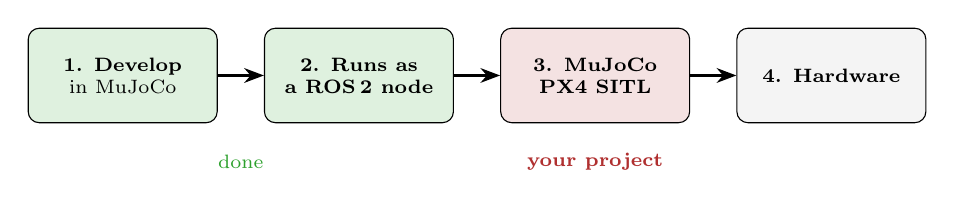
\begin{tikzpicture}[every node/.style={font=\scriptsize},
      st/.style={draw, rounded corners, minimum width=2.4cm, minimum height=1.2cm,
                 align=center},
      done/.style={st, fill=okc!15}, todo/.style={st, fill=warnc!14},
      goal/.style={st, fill=codebg}]
    \node[done] (a) at (0,0)   {\textbf{1. Develop}\\ in MuJoCo};
    \node[done] (b) at (3.0,0) {\textbf{2. Runs as}\\ \textbf{a ROS\,2 node}};
    \node[todo] (c) at (6.0,0) {\textbf{3. MuJoCo}\\ \textbf{PX4 SITL}};
    \node[goal] (d) at (9.0,0) {\textbf{4. Hardware}};
    \foreach \x/\y in {a/b, b/c, c/d}
      \draw[-{Stealth[length=2.5mm]}, thick] (\x) -- (\y);
    \node[font=\scriptsize\color{okc}] at (1.5,-1.1) {done};
    \node[font=\scriptsize\color{warnc}] at (6.0,-1.1) {\textbf{your project}};
  \end{tikzpicture}
  \end{center}

  \vspace{0.45cm}
  \begin{block}{Why a MuJoCo PX4 SITL rather than Gazebo PX4 SITL}
    {\small Gazebo would give you the PX4 protocol but a \emph{different physics
    engine} --- and once the engine differs you can no longer separate a
    deployment bug from an engine difference. The comparison you just watched
    stops working, right before hardware. \cue{Stage 3 keeps both:} real PX4
    protocol \emph{and} the shared model.}
  \end{block}
\end{frame}

% ---------------------------------------------------------------
\begin{frame}[fragile]{Stage 3: the work, in order}
  \begin{enumerate}
    \setlength{\itemsep}{0.24cm}
    \item NED $\leftrightarrow$ ENU and FRD $\leftrightarrow$ FLU conversion,
      with a test asserting a round-trip is the identity
    \item \texttt{OffboardControlMode} heartbeat, \texttt{VehicleCommand}
      arm / mode sequencing
    \item newtons $\to$ normalised \texttt{ActuatorMotors}, calibrated against
      the airframe
    \item run it against real PX4 SITL + Gazebo
    \item takeoff, land, failsafe
  \end{enumerate}

  \vspace{0.4cm}
  \begin{block}{Build it against the MuJoCo SITL first}
    {\small Give the sim node an optional ``PX4 dialect'' and you can test your
    bridge in \emph{one second} per attempt. Gazebo then becomes a confirmation
    step rather than the place you debug sign flips.}
  \end{block}
\end{frame}

% ---------------------------------------------------------------
\begin{frame}[fragile]{It is not as bad as it sounds}
  \cue{The toolchain is already installed on this machine:}

  \vspace{0.3cm}
  \begin{center}
  \small
  \begin{tabular}{@{}ll@{}}
    \toprule
    PX4-Autopilot & source present, \textbf{already built}\\
    Gazebo & 8.9.0 on PATH\\
    \texttt{MicroXRCEAgent} & installed (the PX4 $\leftrightarrow$ ROS\,2 bridge)\\
    \texttt{px4-offboard} & a \textbf{working reference} --- heartbeat, arming,
      setpoints\\
    \bottomrule
  \end{tabular}
  \end{center}

  \vspace{0.4cm}
  {\small There is no clever algorithm in any of this. It is careful bookkeeping
  against a documented protocol.}

  \vspace{0.25cm}
  \begin{alertblock}{What makes it genuinely hard}
    {\small The failures are \emph{silent}. A sign flip does not raise an
    exception --- it crashes the vehicle. There is no stack trace to read, which
    is exactly why it wants tests rather than inspection.}
  \end{alertblock}
\end{frame}

% ---------------------------------------------------------------
\begin{frame}[fragile]{Running it yourself --- setup}
\begin{lstlisting}
# 1. you need your own PX4 workspace with px4_msgs built
export PX4_WS=/path/to/your/px4_ws

# 2. sanity check -- nothing to build, the nodes run as plain
#    Python processes once ROS is sourced
cd ~/mjc_sitl_px4
python3 -m mjc_sitl parity          # expect 12/12
python3 -m pytest mjc_sitl/tests -q # expect 22 passed
\end{lstlisting}

  \vspace{0.3cm}
  {\small Requirements: Python 3.10, ROS\,2 Humble, \texttt{mujoco>=3.3},
  \texttt{numpy}, \texttt{scipy}, \texttt{px4\_msgs}. Optional:
  \texttt{matplotlib} + \texttt{mediapy} for figures and video.}

  \vspace{0.2cm}
  {\small On a headless machine, prefix rendering commands with
  \texttt{MUJOCO\_GL=egl}.}
\end{frame}

% ---------------------------------------------------------------
\begin{frame}[fragile]{Running it yourself --- the three commands}
\begin{lstlisting}
./demo.sh parity   # do sim and SITL share physics?        (5 s)
./demo.sh fly      # figure-8 in sim AND ROS 2, compare   (~90 s)
./demo.sh show     # open the pre-generated artifacts     (instant)
\end{lstlisting}

  \vspace{0.3cm}
  Or drive it directly:

\begin{lstlisting}
python3 -m mjc_sitl compare --controller pd --task figure8 \
    --duration 24 --tier full --outdir demo/figure8
\end{lstlisting}

  \vspace{0.25cm}
  {\small \texttt{--controller} takes \texttt{pd}, \texttt{mpc}, \texttt{ppo} or
  \texttt{mine}; \texttt{--task} takes \texttt{hover} or \texttt{figure8}.
  \texttt{--tier fast} skips ROS entirely and runs in about a second, which is
  what you want while iterating.}

  \vspace{0.25cm}
  {\small Stuck on something that looks like physics? Run \texttt{parity}
  first. If it says 12/12, the airframe is not your problem.}
\end{frame}

% ---------------------------------------------------------------
\begin{frame}[fragile]{Where to look}
  \begin{center}
  \begin{tabular}{@{}ll@{}}
    \toprule
    \file{README.md} & what it does, what it cannot do, where it goes\\
    \file{sim\_mjc/CLAUDE\_SIM.MD} & how the simulator works\\
    \midrule
    \file{mjc\_sitl/scenegen.py} & the shared scene --- the whole idea, 150 lines\\
    \file{mjc\_sitl/bridge.py} & frames, units, rotor order\\
    \file{mjc\_sitl/offboard\_lib/} & the two ROS\,2 nodes\\
    \bottomrule
  \end{tabular}
  \end{center}

  \vspace{0.7cm}
  {\small The airframe is defined \emph{once}, in
  \file{sim\_mjc/sim\_mjc/config.py:DRONE}. Change it there and run
  \texttt{python3 -m mjc\_sitl sync} --- never edit the generated copies by
  hand.}
\end{frame}

% ---------------------------------------------------------------
{\setbeamertemplate{footline}{}
\begin{frame}
  \vspace{1.0cm}
  \begin{center}{\Large\bfseries Three things}\end{center}
  \vspace{0.7cm}
  \begin{enumerate}
    \setlength{\itemsep}{0.45cm}
    \item {\large Sim and SITL run the \textbf{same compiled model}.}\\
      {\small So a difference between them is a deployment bug, never physics.}
    \item {\large It is \textbf{not} PX4-ready. The frame flip alone is fatal.}\\
      {\small That gap is stage 3 --- and it is the project.}
    \item {\large Build stage 3 \textbf{against MuJoCo first}.}\\
      {\small One-second feedback beats debugging sign flips in Gazebo.}
  \end{enumerate}
  \vspace{0.8cm}
  \begin{center}{\color{dimc} Start with \file{README.md}, then \texttt{./demo.sh show}.}\end{center}
\end{frame}}

\end{document}
